\section{Results} %Movido para arquitetura e conclusao

Our team performed very well and we won the MAPC for the second consecutive year. The strategy to get many small zones was the strongest point of our team and it became more difficult for the opponents to disturb our zones since our agents were spread out over the whole map while our saboteurs were able to disturb the opponent zones. However, our team can be improved to perform better in maps with low thinning (less than 20\%) and with too many good vertices gathered in the same place. In that case, the best strategy seems to be to build a big zone and defend it instead of building just small zones.

\begin{figure}[th]
 \centering
 \subfigure[Scores]{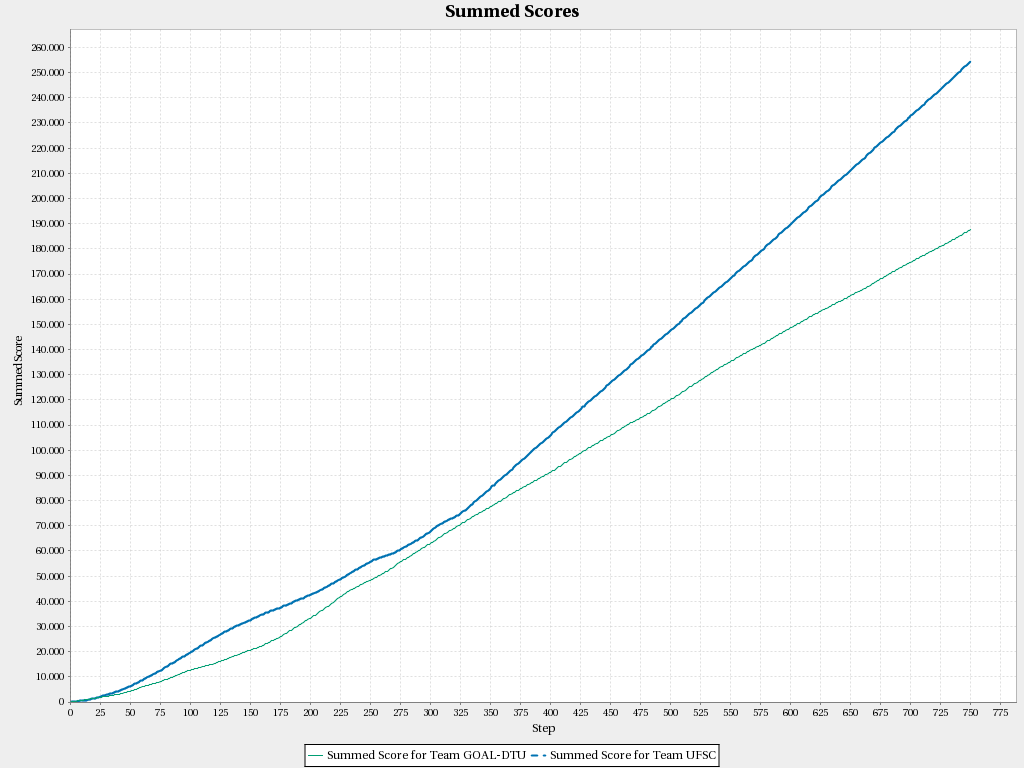
\includegraphics[width=0.49\textwidth]{figs/Scores.png}\label{fig:Scores}}
 \subfigure[ZoneStabilities]{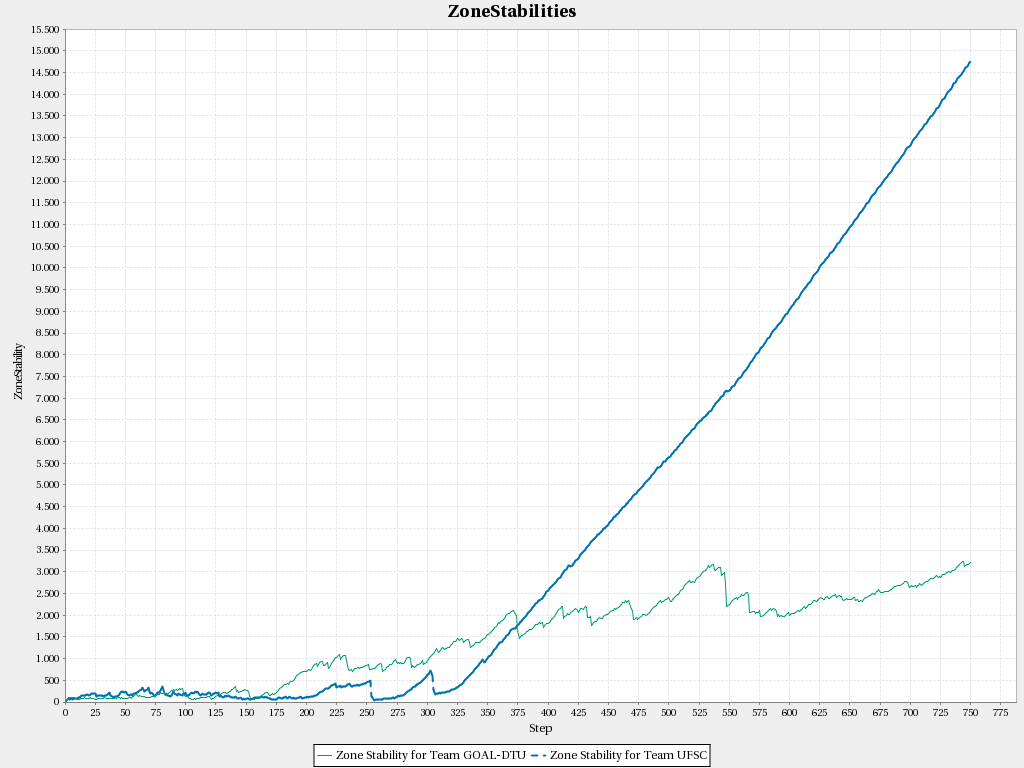
\includegraphics[width=0.49\textwidth]{figs/ZoneStabilities.png}\label{fig:ZoneStabilities}}
 \\
 \subfigure[AchievementPoints]{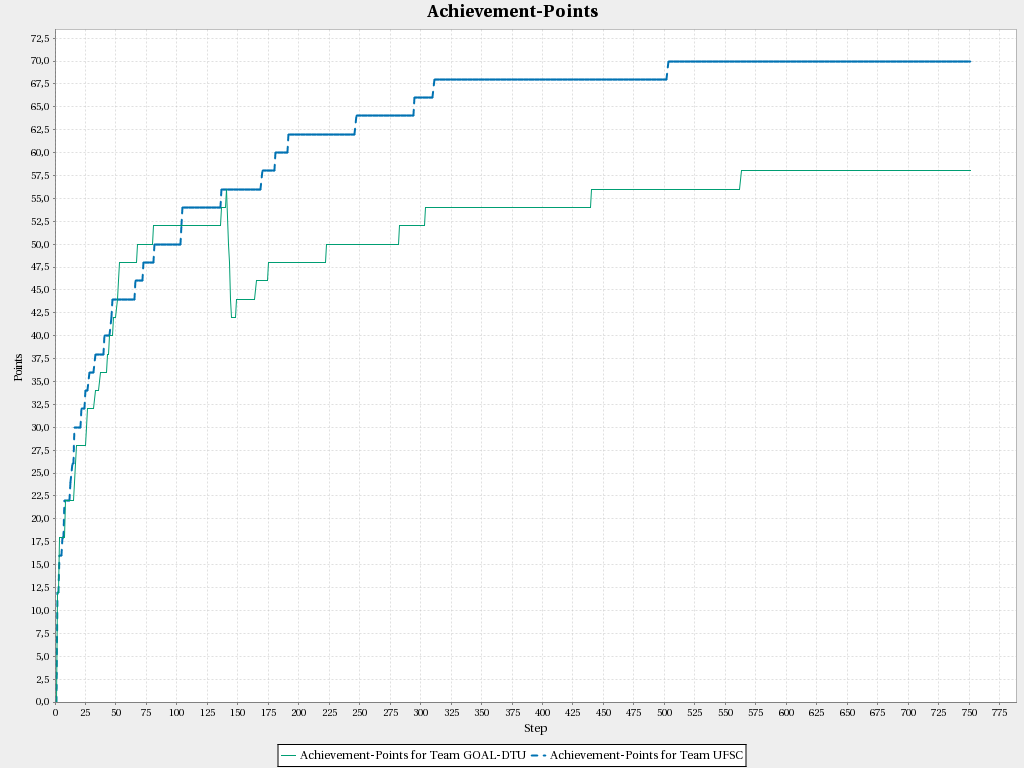
\includegraphics[width=0.49\textwidth]{figs/AchievementPoints.png}\label{fig:AchievementPoints}}
 \subfigure[ZonesScores]{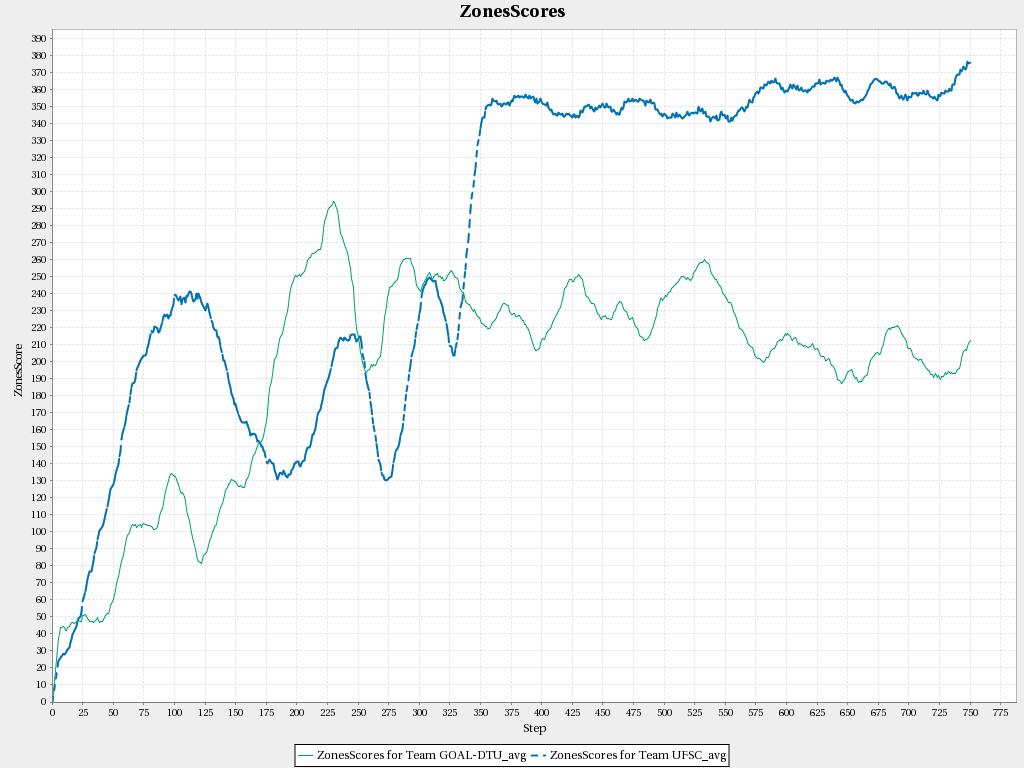
\includegraphics[width=0.49\textwidth]{figs/ZonesScores.png}\label{fig:ZonesScores}} 
 \caption{Statistics}
 \label{fig:statistics}
\end{figure}

In order to highlight the main results of our strategy we chose to use some statistics of the second match against the GOAL-DTU team \footnote{\url{http://multiagentcontest.org/downloads/func-startdown/1716/}}, which got the second place. Due our strategy of small zones, we can verify in the Fig.~\ref{fig:ZoneStabilities}  that after step 325 our team (blue) kept almost the same zones until the end of the match. This behavior is usual in all matches against the other teams. The reason is that no matter what the opponent does, our agents will rarely leave their positions.

Another interesting result can be drawn from the zones scores plot (Fig.~\ref{fig:ZonesScores}). We can see that our team (blue) kept getting almost the same zone scores after step 350 and always more than the opponent. The phase of hills can also be noticed in the beginning of the match, between step 25 until around step 130, where the team is getting high scores because of the big zones. After step 130 our team started to conquer small zones (pivots and islands) and, therefore, spreading the agents out over the whole map. It is also possible to see that, sometimes, our zone scores were lower than the enemies. This was an expected behavior when the agents were still changing their positions because the explorers were still probing new vertices. We can see it after step 250 and after around step 315, where our team decreased the gain of zone scores. After probing all vertices (around step 325), the agents started to get higher scores because they defined the fixed zones and all agents were participating.

We can see the same behavior in Fig.~\ref{fig:Scores}, where the opponent score gets closer and then the difference of scores increases again. Notice that after step 325 the difference of scores increased continuously because all vertices were probed. On the other hand, in the Fig.~\ref{fig:AchievementPoints} we can see that our team always has more achievement points than the opponent after step 125. It means we are getting more points because the opponent was buying items while our team was saving money.

\bigskip

Besides the performance of the team in the contest, we made several contributions for the tools that we used in this year. In Jason, we added features to handle goals with deadlines, new mechanisms for the \texttt{.wait} internal action, and we fixed some bugs. In \moise, we added a new feature to reset organizational goals to avoid creating new schemes at runtime and we added an organizational monitor accessed via HTTP, so that we were able to watch our team organization remotely.


The source code of the team has 3794 lines of Jason code, 135 for \moise, 96 for \cartago, and 4434 for Java, totaling 8459 lines. Although the implemented strategies of these year are more complex, we can notice that the number of lines coded in Jason has decreased from 5504 in last year's team to 3794 this year. It is an expected consequence of the organization and the environment programming available in \jacamo. Coordination strategies that previously required several lines of Jason code, could now be coded in a few lines of \moise, since \moise\ is a proper language for that.  Not only have we reduced the size of the programs, but the new approach has allowed us to debug and change the organization of the team quite easily. Instead of monitoring the agents internal state, we can now monitor the state of the organization, which is a more general view of the state of the team. Since the organizational program is the same as the specification, to change the team sometimes is simply reduced to update the organization. For instance, to change the order of organizational goals, we simply need to change the scheme of Fig.~\ref{fig:org_fs}.